\documentclass{article}

% includes
\usepackage{graphicx}
\usepackage{enumitem}
\usepackage{amsmath}
\usepackage[margin=1in]{geometry}
\usepackage{listings}
\usepackage{xcolor}
\usepackage{amsfonts} 
\usepackage{float}
\usepackage{booktabs}
\usepackage{subcaption}
\usepackage{hyperref}
\usepackage{cleveref}

% for matlab code

\lstset{
	language=Matlab,
	basicstyle=\ttfamily\small,
	keywordstyle=\color{blue},
	commentstyle=\color{gray},
	stringstyle=\color{red},
	backgroundcolor=\color{white},
	showspaces=false,
	showstringspaces=false,
	frame=single,
	breaklines=true
}

% Set-shorts
\newcommand{\N}{\ensuremath{\mathbb{N}}}   % natural numbers
\newcommand{\Z}{\ensuremath{\mathbb{Z}}}   % integers
\newcommand{\Q}{\ensuremath{\mathbb{Q}}}   % rationals
\newcommand{\R}{\ensuremath{\mathbb{R}}}   % real numbers
\newcommand{\C}{\ensuremath{\mathbb{C}}}   % complex numbers
\newcommand{\vrel}{\ensuremath{v_{\text{rel}}}} % for one example


\title{Exercises: Introductory Course on Implicitly Switched ODEs and Filippov Sliding}
\author{Andreas Sommer, Lev Gromov, Marvin Hertweck, Pilar Keller}
\date{July 09, 2026}

\begin{document}
\maketitle
% !TeX root = solutions_main.tex
\section*{Task 1: Solution}
\begin{enumerate}[label=\alph*)]
    \item\label{item:task1a} The solution computed by \lstinline|ode45| is incorrect. The second component should have a bend when the first component crosses the $750$ threshold.

	The integrator \lstinline|ode45| can only be used to solve smooth systems. The switched system, however, contains discontinuities in the RHS. Since the system violates a key requirement of \lstinline|ode45|, we cannot expect to receive a correct solution. The integrator \lstinline|ode45| is simply not designed to solve these types of switched problems.
	
	For this particular example, the integrator takes large steps because the system is smooth at the beginning. Due to the large step size, the integrator completely misses the discontinuity (which it has no way of knowing about since the RHS is assumed to be smooth).\\\\
    \textbf{File:} \texttt{rhsTask1.m}
    \begin{lstlisting}
function dy = rhsTask1(t, y, p)
dy = zeros(2, 1);

q1 = 50/27*t^2 - 100/3*t + 400/3;
q2 = (1000-y(2)) * (p(1)*(t-19) + p(2));

if y(1) <= 750
    dy(1) = q1;
    dy(2) = 0;
elseif y(1) < 800
    dy(1) = q1 - q2;
    dy(2) = -300;
else
    dy(1) = q1 - q2;
    dy(2) = 0;
end
end
    \end{lstlisting}
    \textbf{File:} \texttt{runTask1.m}
    \begin{lstlisting}
%% Subtask a) and b)
%% Setup problem
tspan = [0, 30];
y0 = [0; 1000];
p = [3/4, 1/4];

rhs = @rhsTask1a;
integrator = @ode45;
optionsOde45 = odeset('RelTol', 1e-8, 'AbsTol', 1e-8);

%% Solve with ode45
solutionOde45 = integrator(@(t, y) rhs(t, y, p), tspan, y0, optionsOde45);

%% Plot solution
t = linspace(tspan(1), tspan(end), 1000);
yOde45 = deval(solutionOde45, t);

figure;
plot(t, yOde45);
title('Solution with ode45');
    \end{lstlisting}
    \begin{figure}[H]
        \centering
        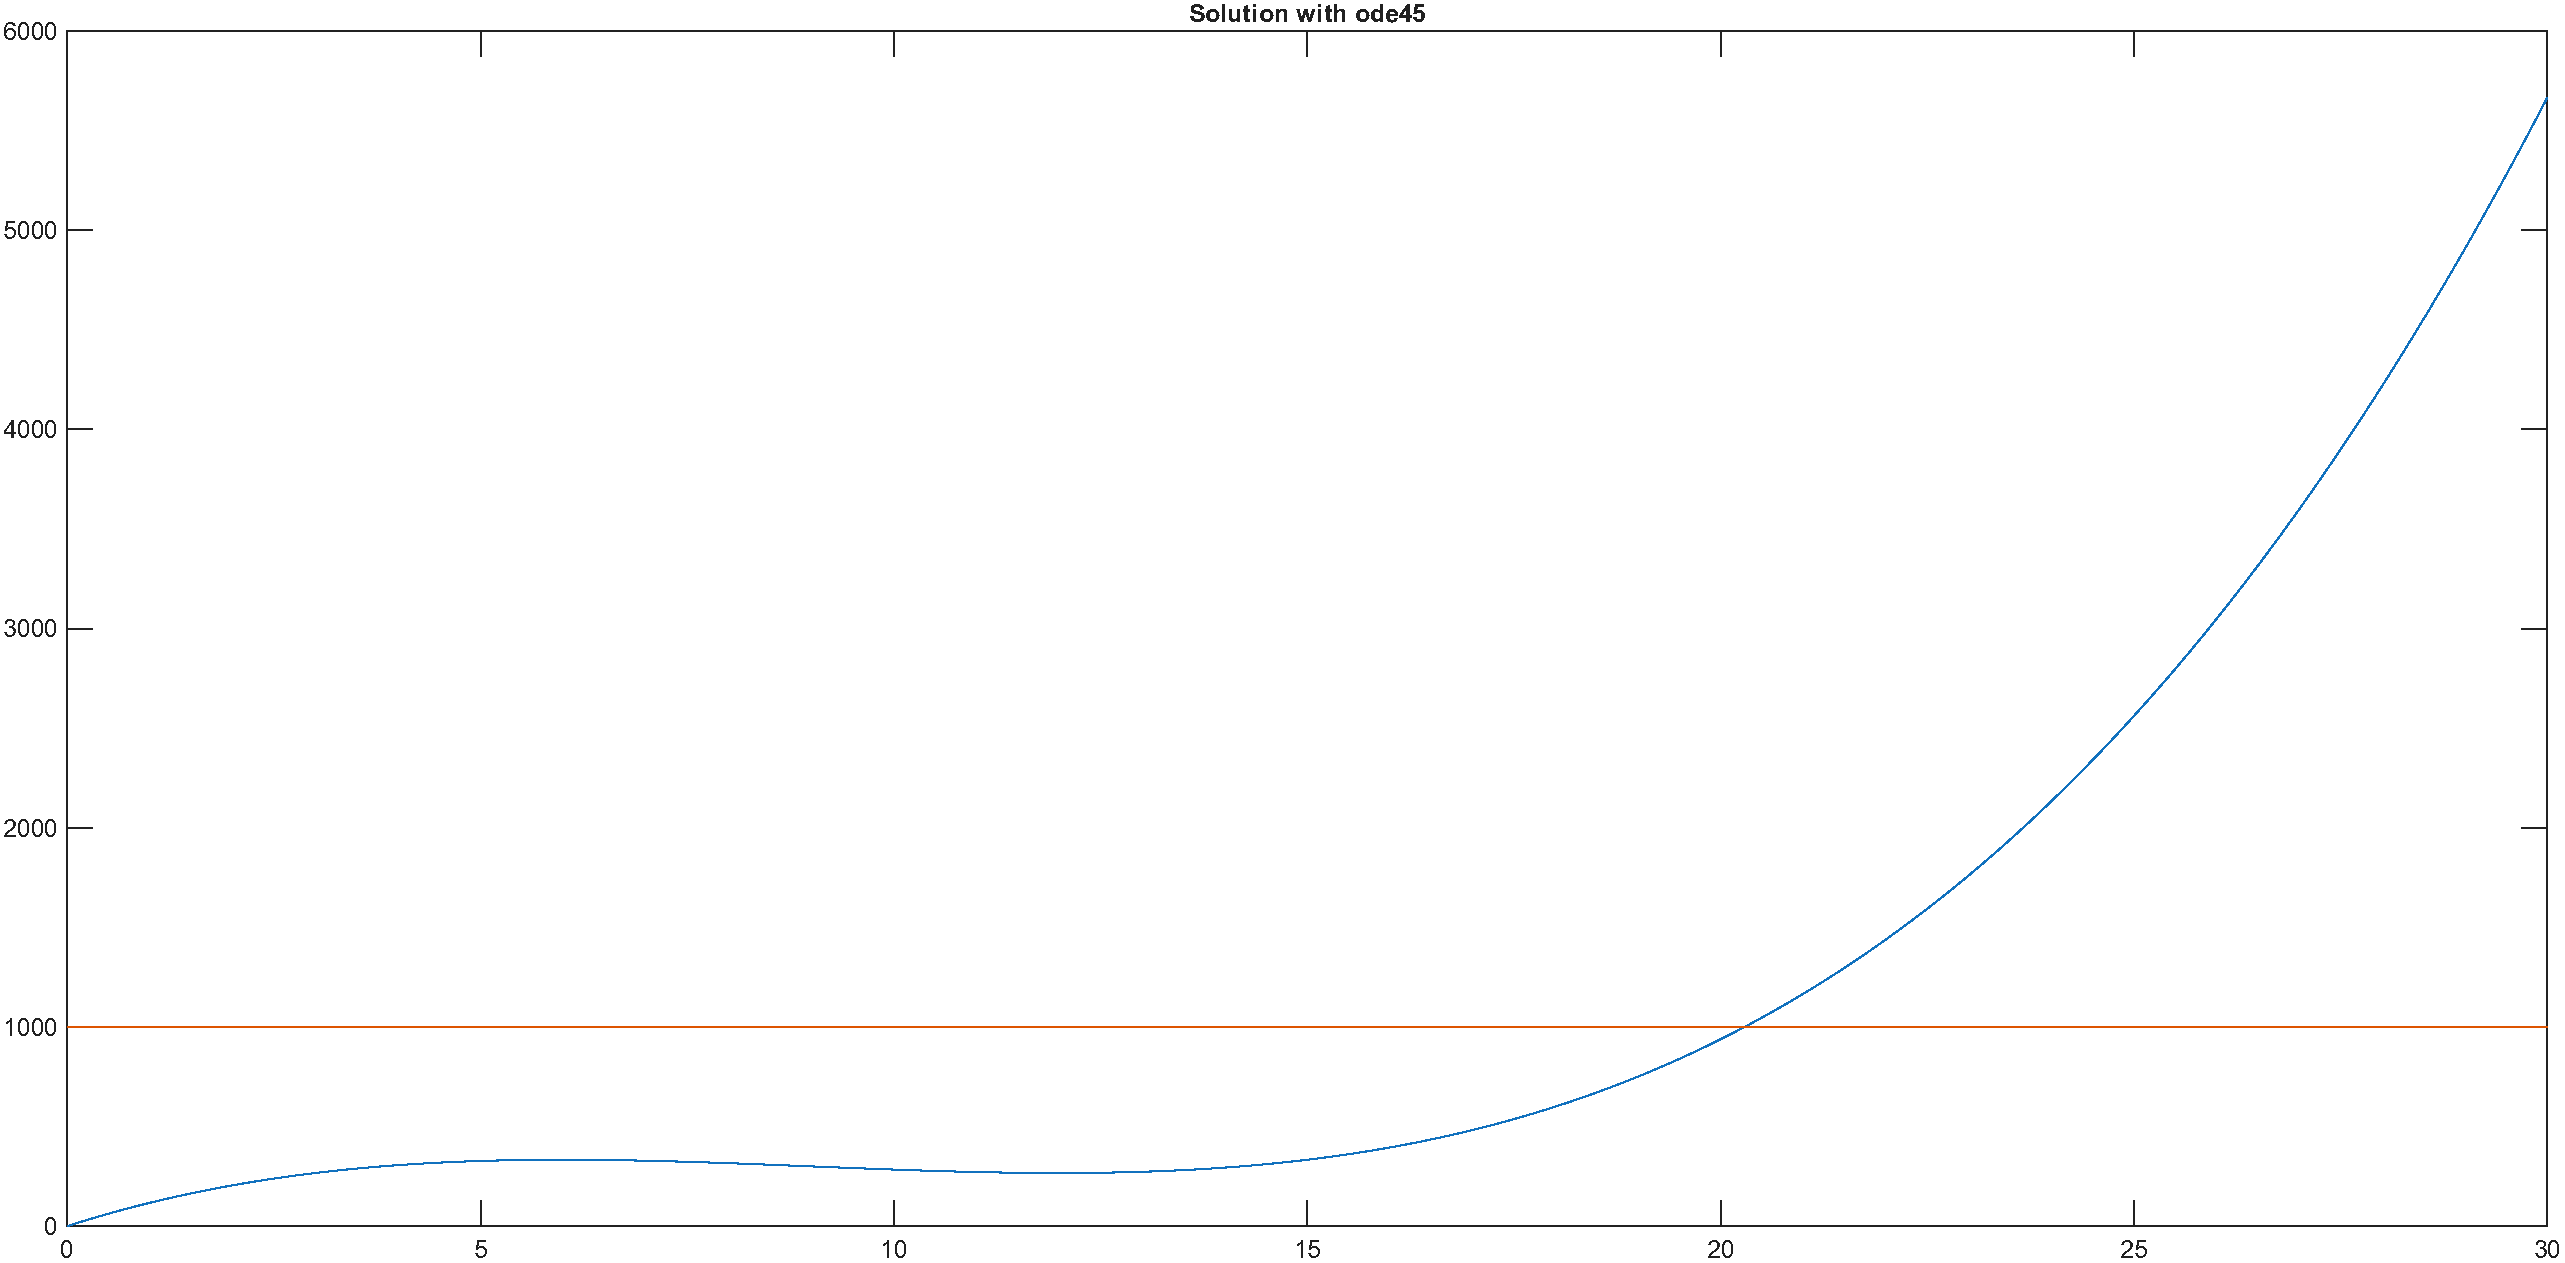
\includegraphics[width=\textwidth]{Plots/task1a}
        \caption{\textbf{Incorrect} solution plot with ode45 for subtask \ref{item:task1a}}
    \end{figure}

    \item\label{item:task1b} The solution produced by \lstinline|ode45| with a maximum integration step size of $0.1$ is correct. We can see the characteristic bend of the second solution component which was missing in the plot from subtask \ref{item:task1a}.
	
	By forcing the integrator to take tiny steps, it manages to approximate the non-smooth regions of the solution through sheer brute force.
	
	However, this approach has multiple faults: For one, there is no way to know beforehand how small the maximum step size should be to ensure that the integrator manages to compute the correct solution. Secondly, enforcing a tiny step size will massively drive up computation time and completely defeats the purpose of using an adaptive step size integrator like \lstinline|ode45| in the first place. Finally, it is not possible to compute sensitivities with this approach, as will be shown in subtask \ref{item:task1d}. \\\\
    \textbf{File:} \texttt{runTask1.m}
    \begin{lstlisting}
%% Subtask a) and b)
%% Setup problem
tspan = [0, 30];
y0 = [0; 1000];
p = [3/4, 1/4];

rhs = @rhsTask1a;
integrator = @ode45;
optionsOde45 = odeset('RelTol', 1e-8, 'AbsTol', 1e-8, 'MaxStep', 0.1);

%% Solve with ode45
solutionOde45 = integrator(@(t, y) rhs(t, y, p), tspan, y0, optionsOde45);

%% Plot solution
t = linspace(tspan(1), tspan(end), 1000);
yOde45 = deval(solutionOde45, t);

figure;
plot(t, yOde45);
title('Solution with ode45');
    \end{lstlisting}
    \begin{figure}[H]
        \centering
        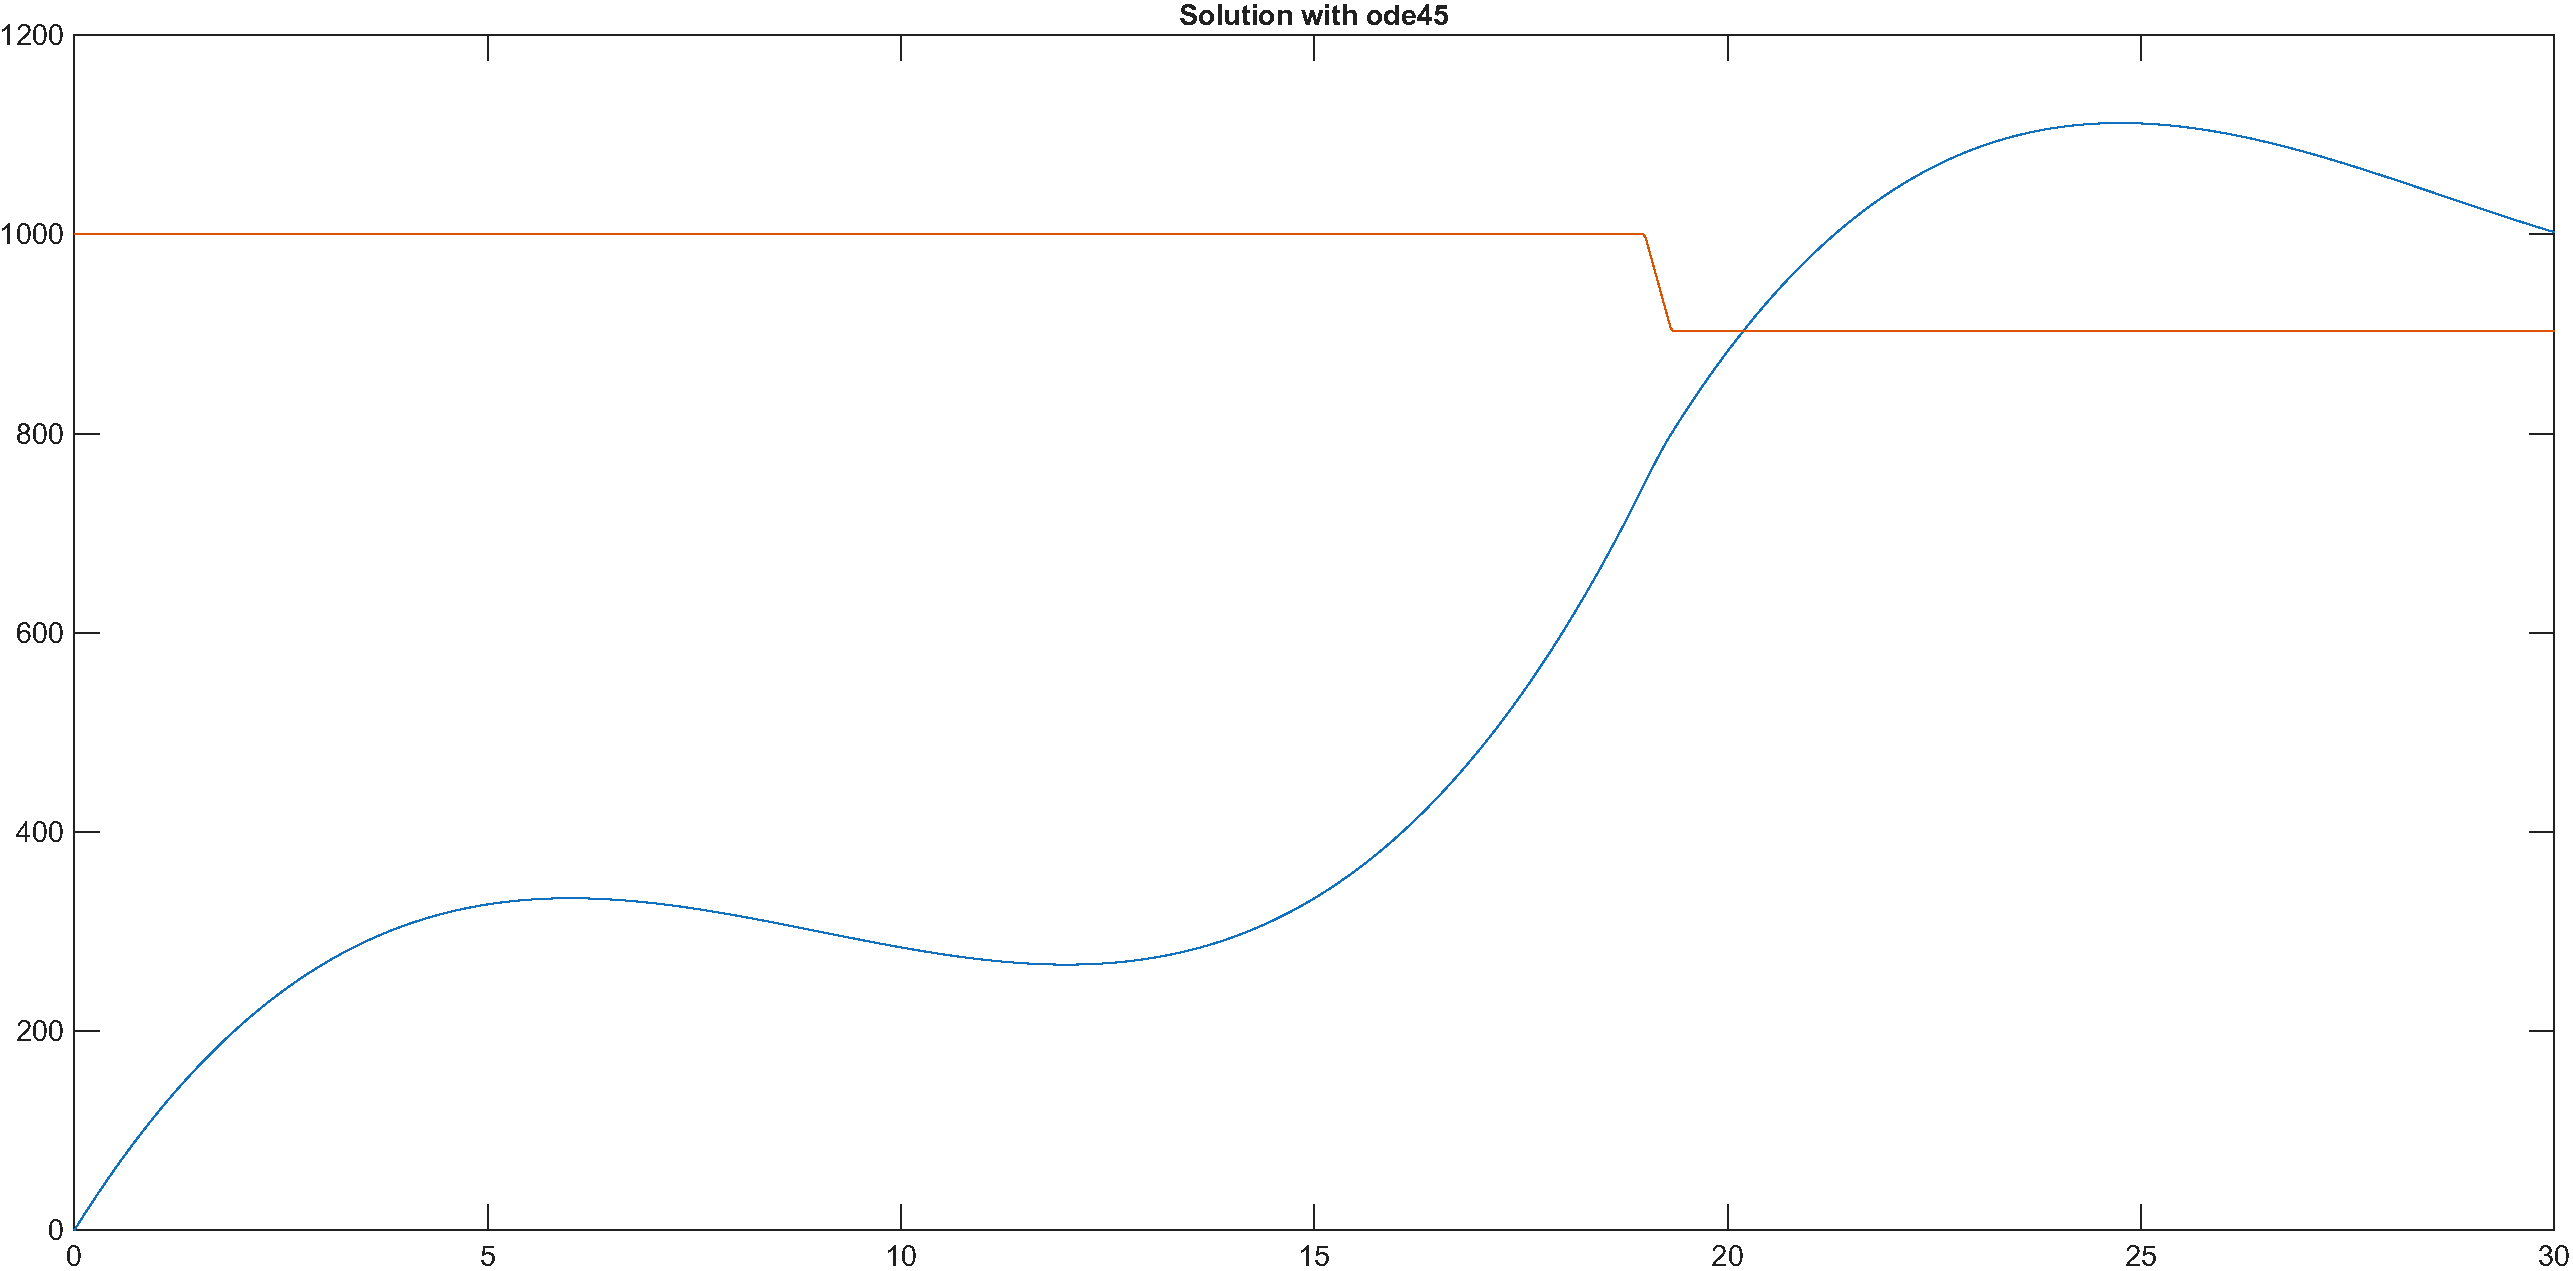
\includegraphics[width=\textwidth]{Plots/task1b}
        \caption{Solution plot with ode45 (maximum step size 0.1) for subtask \ref{item:task1b}}
    \end{figure}

    \item\label{item:task1c} The correct solution produced by IFDIFF matches the solution from subtask \ref{item:task1b}.
    
	Unlike \lstinline|ode45|, IFDIFF is designed to handle switched systems and can thus take full advantage of adaptive step size integrators like \lstinline|ode45| to compute the solution accurately and efficiently.\\\\
    \textbf{File:} \texttt{runTask1.m}
    \begin{lstlisting}
%% Subtask c)
%% Setup problem for IFDIFF
optionsIfdiff = odeset('RelTol', 1e-8, 'AbsTol', 1e-8);
datahandle = prepareDatahandleForIntegration(rhs, 'integrator', integrator, 'options', optionsIfdiff);

%% Solve with IFDIFF
solutionIfdiff = solveODE(datahandle, tspan, y0, p);

%% Plot solution
t = linspace(tspan(1), tspan(end), 1000);
yIfdiff = deval(solutionIfdiff, t);

figure;
plot(t, yIfdiff);
title('Solution with IFDIFF');
    \end{lstlisting}
    \begin{figure}[H]
        \centering
        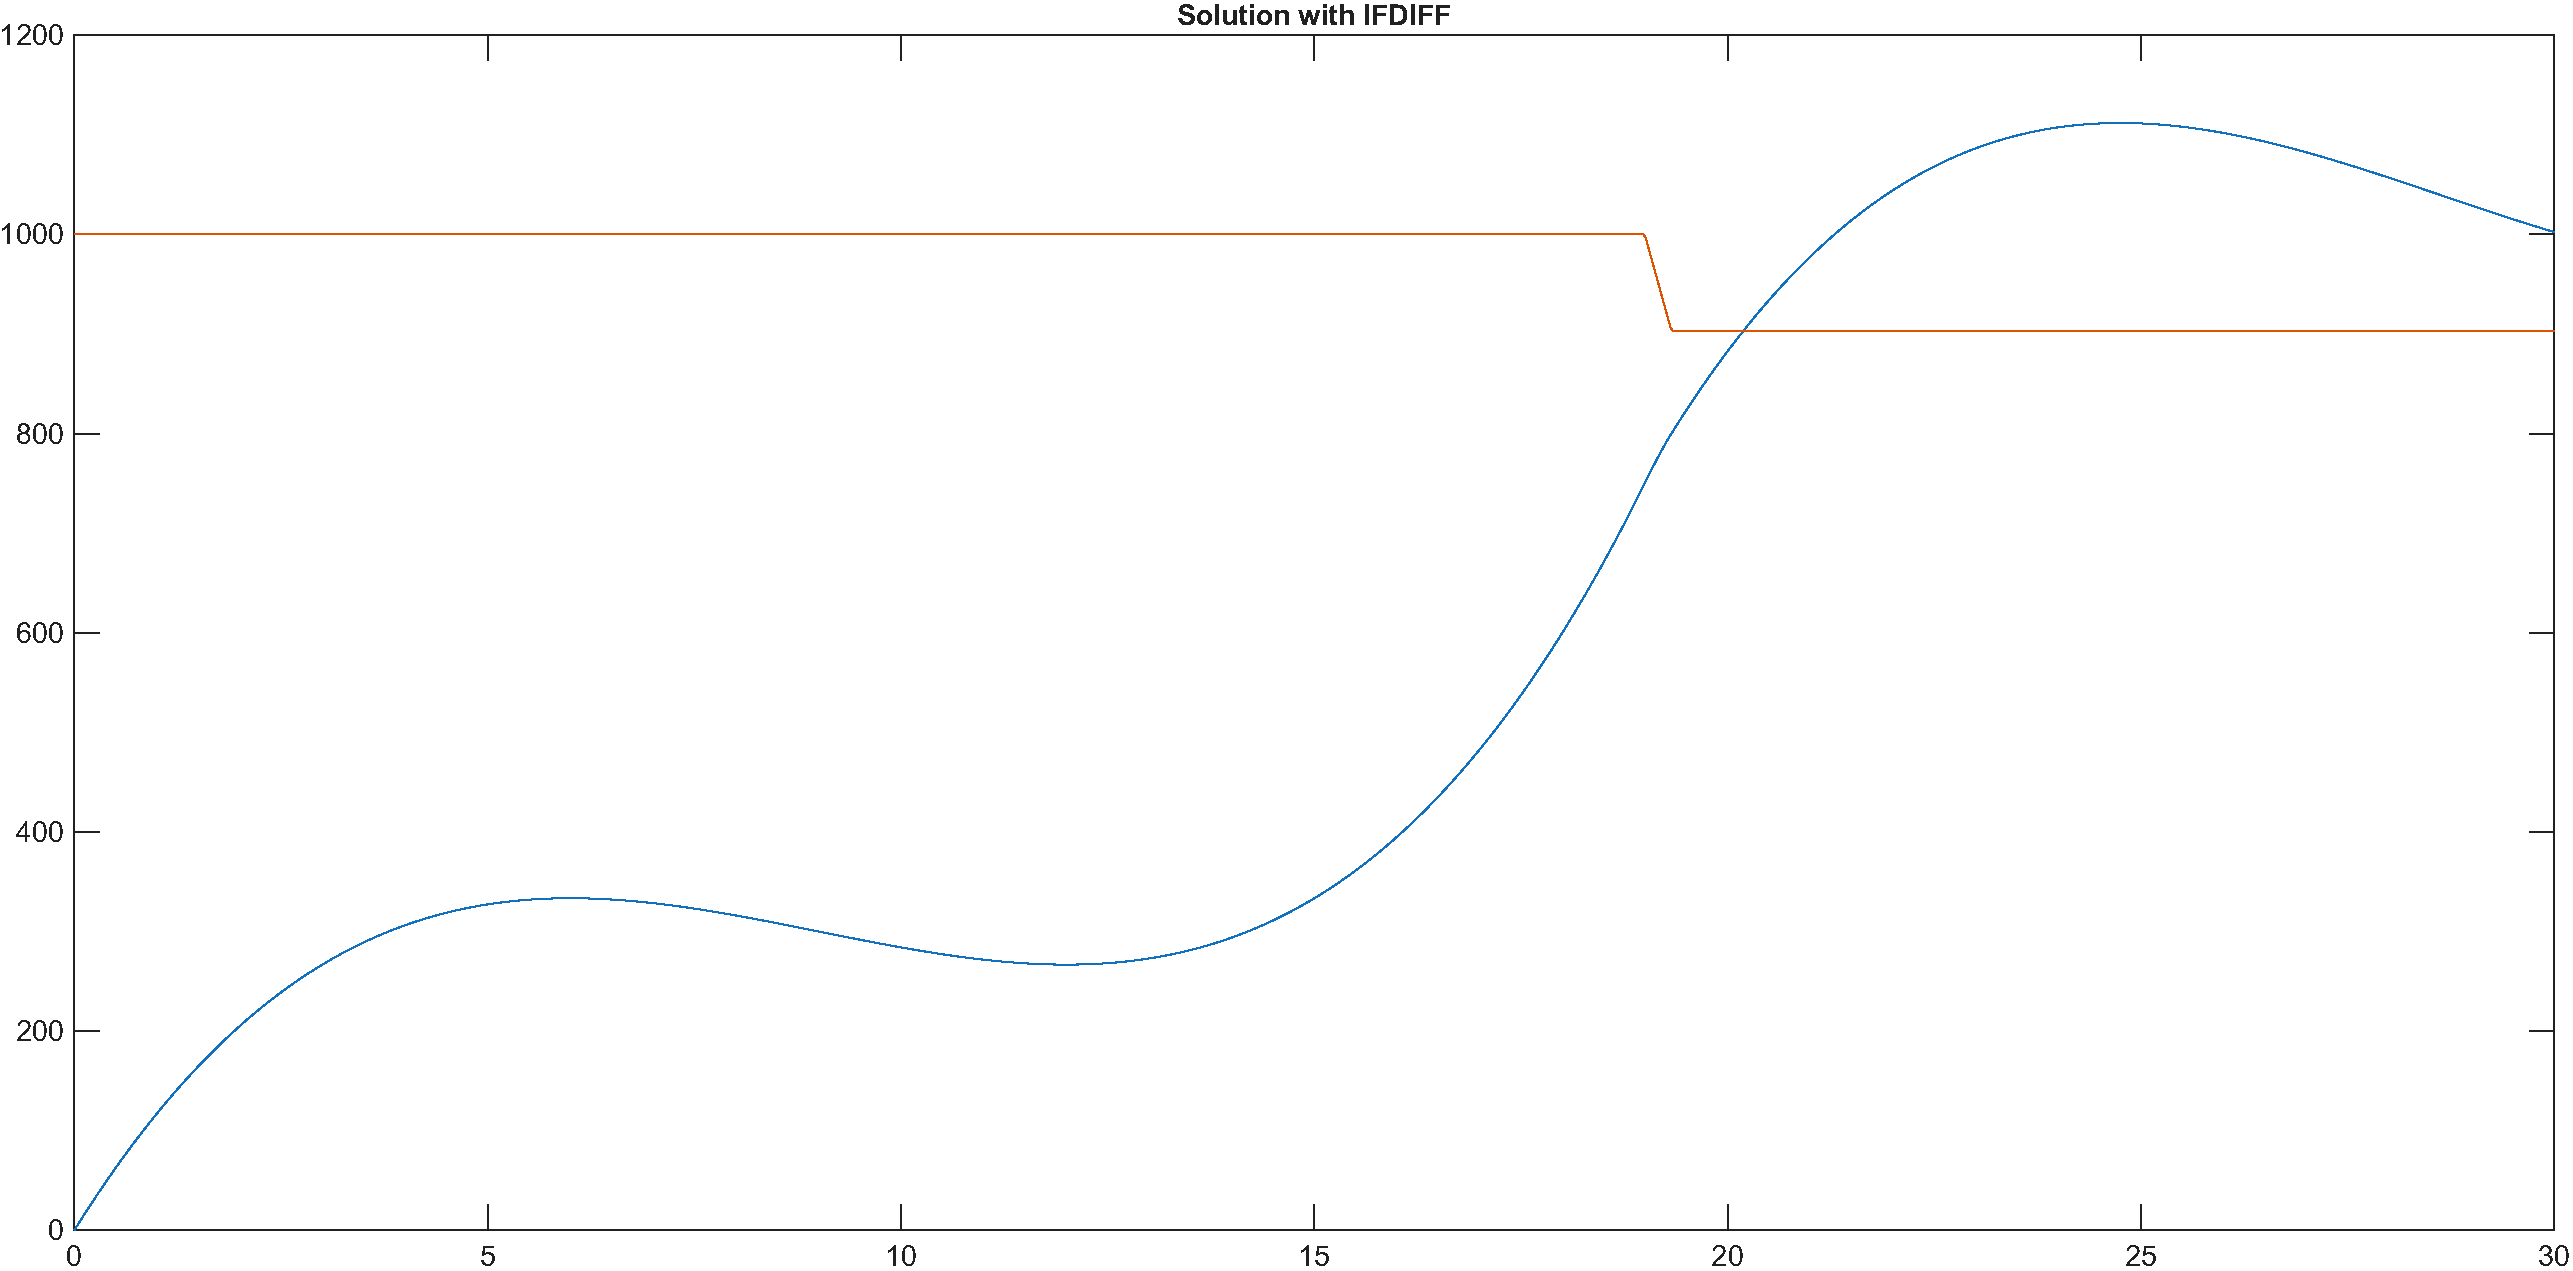
\includegraphics[width=\textwidth]{Plots/task1c}
        \caption{Solution plot with IFDIFF for subtask \ref{item:task1c}}
    \end{figure}

    \item\label{item:task1d} The sensitivities derived from the solution computed by \lstinline|ode45| are incorrect.
    
	Take $G_y(1,1)$ as an example, which describes how the first solution component changes with respect to changes in its initial value. The sensitivity before the first switch is one, which is correct because the derivative of the first solution component does not depend on the state of the first solution component, so shifting the initial value will shift the whole solution by the same amount. However, increasing the first solution component would trigger the switch earlier because $y_1(t)$ would hit the threshold $750$ quicker. Therefore, we would expect to see a sharp downwards bend in the sensitivity at the switch since the second solution component activates there and massively dampens the growth of the first solution component. This bend is completely absent in the incorrect sensitivity derived from the solution computed by \lstinline|ode45|. \\\\
    \textbf{File:} \texttt{runTask1.m}
    \begin{lstlisting}
%% Subtask d)
%% Compute sensitivity with ode45
t = linspace(tspan(1), tspan(end), 1000);
sensitivityOde45 = computeSensitivityOde45(solutionOde45, t);

%% Plot sensitivity
plotSensitivity(sensitivityOde45);
    \end{lstlisting}
    \begin{figure}[H]
        \centering
        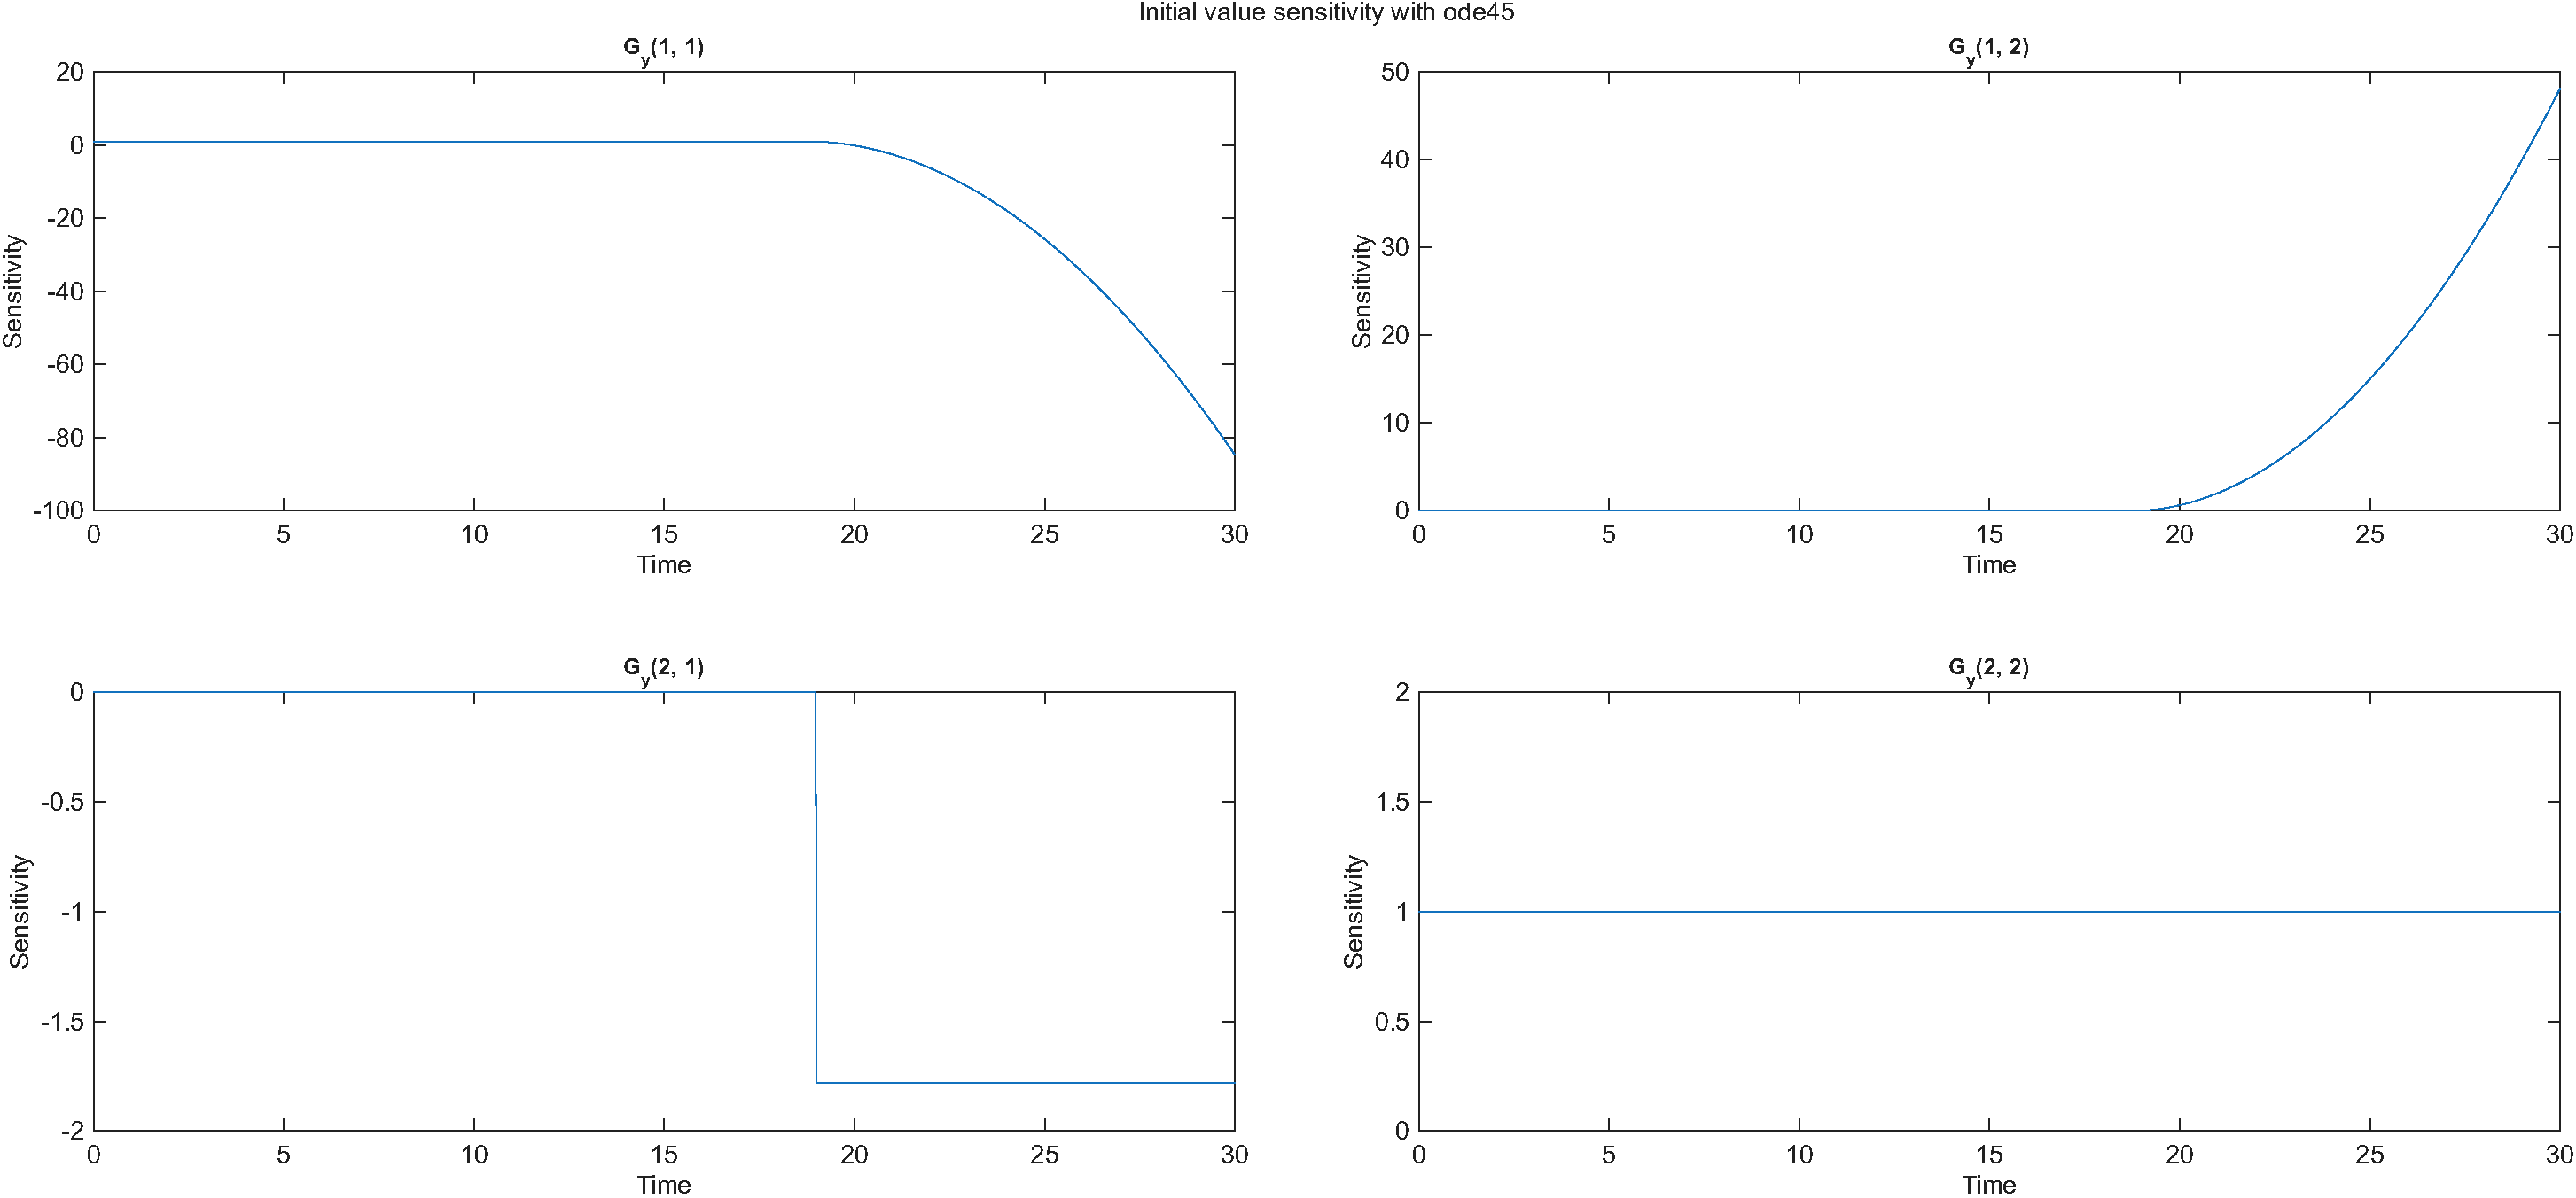
\includegraphics[width=\textwidth]{Plots/task1d}
        \caption{\textbf{Incorrect} sensitivity plot with ode45 for subtask \ref{item:task1d}}
    \end{figure}

    \item\label{item:task1e} The sensitivities computed by IFDIFF are correct.
    
	We can see the characteristic downward bend in the plot for $G_y(1,1)$, which was missing in the incorrect sensitivities from subtask \ref{item:task1d}. \\\\
    \textbf{File:} \texttt{runTask1.m}
    \begin{lstlisting}
%% Subtask e)
%% Compute sensitivity with IFDIFF
t = linspace(tspan(1), tspan(end), 1000);

sensitivityFunction = generateSensitivityFunction(datahandle, solutionIfdiff, 'calcGp', false);
sensitivityIfdiff = sensitivityFunction(t);
    \end{lstlisting}
    \begin{figure}[H]
        \centering
        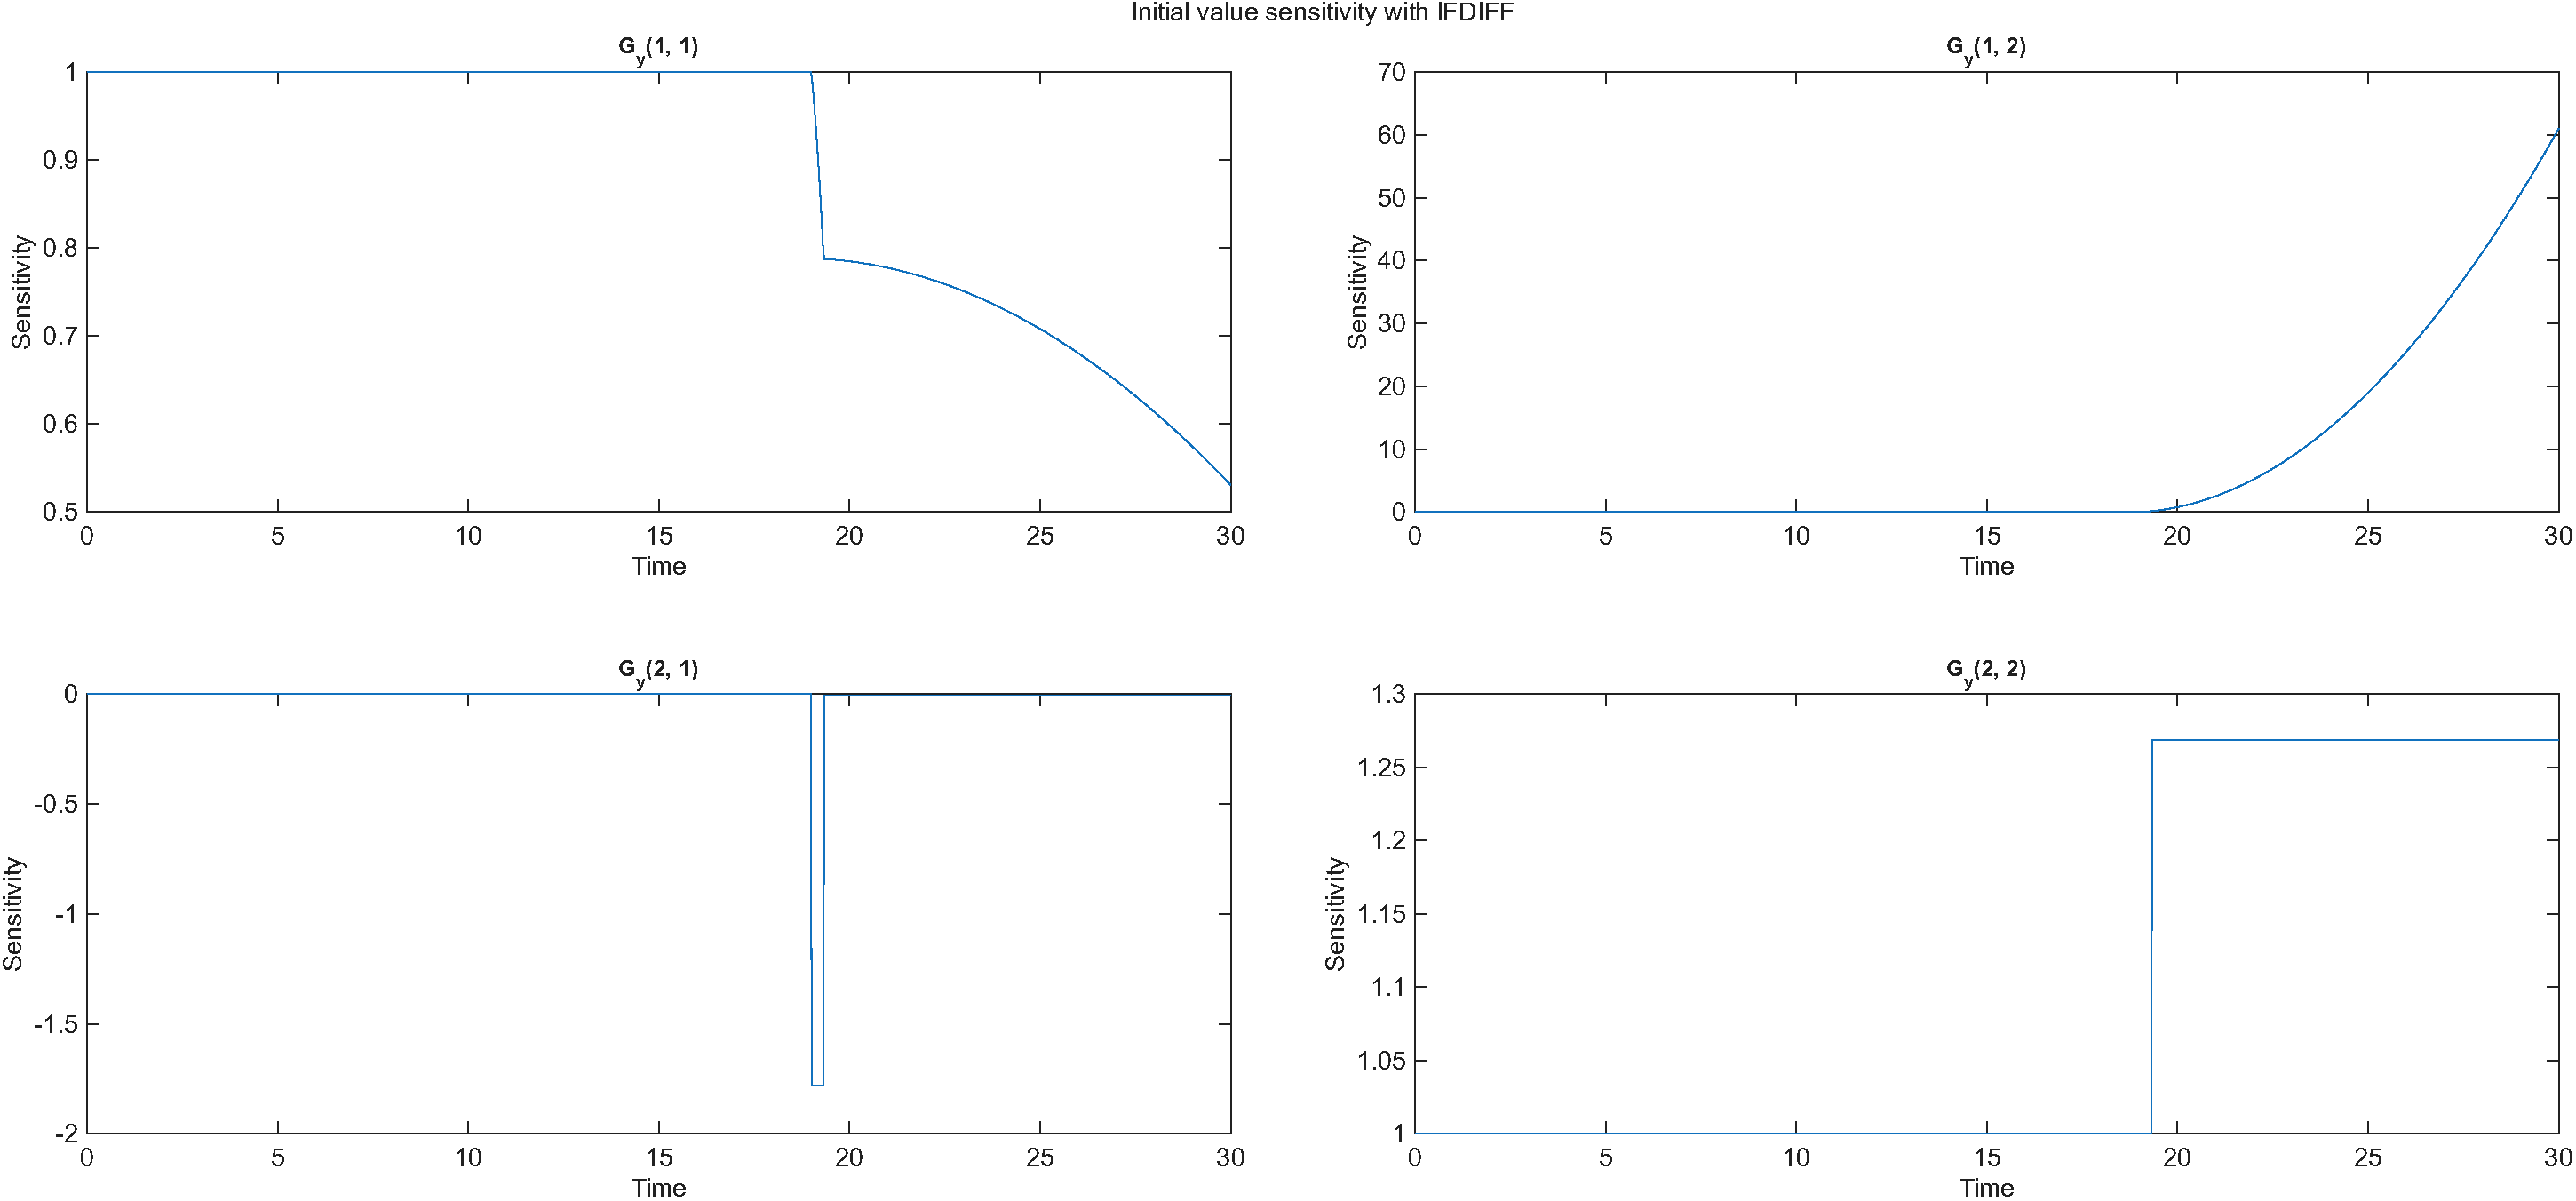
\includegraphics[width=\textwidth]{Plots/task1e}
        \caption{Sensitivity plot with IFDIFF for subtask \ref{item:task1e}}
    \end{figure}
\end{enumerate}
 % Fundamentals
\newpage
%% !TeX root = solutions_main.tex

\section*{Solution 2: Stick Slip (Filippov Behaviour)}
\begin{enumerate}[label=\alph*)]
\item \textbf{Right-hand side} 
\newline
File name: \texttt{rhsTask2Fil.m}
\begin{lstlisting}
function dx = rhsTask2Fil(t, x, p)
% p = (k, m, v_b, F_s, delta, epsilon)
k       = p(1);
m       = p(2);
v_b     = p(3);
F_s     = p(4);
delta   = p(5);
epsilon = p(6);
v_rel   = x(2) - v_b;

dx = zeros(2,1);
dx(1) = x(2);

dx(2) = -(k / m) * x(1) + F_fil(v_rel, F_s, delta) / m;
end
\end{lstlisting}
File name: \texttt{F\_fil.m}
\begin{lstlisting}
function res = F_fil(v_rel, F_s, delta)
  if v_rel <= 0
    res = F_s / (1 - delta * v_rel);
  end
  if v_rel > 0
    res = -F_s / (1 + delta * v_rel);
  end
end
\end{lstlisting}

\noindent
Now, the main executable file can be modified and called. Here shown are only the relevant sections. Find the full \texttt{.m} file in the Heibox:
File name: \texttt{runTask2.m}
\begin{lstlisting}
% ...
%% Model setup
tspan = [0, 30];
y0 = [1; 0];
k       = 1.0;      % spring constant
m       = 1.0;      % mass
v_b     = 0.2;      % velocity relative to the conveyerbelt
F_s     = 1.0;      % max static friction force
delta   = 3.0;      % Physics constant
epsilon = 1e-10;    % numerical zero parameter
p = [k, m, v_b, F_s, delta, epsilon];

% ...

%% Solving the friction model variant with sliding mode
slidingRhs = @rhsTask2Fil;
slidingDatahandle = prepareDatahandleForIntegration(slidingRhs,... 
	'integrator', integrator,... 
	'options', optionsOde);
slidingSol = solveODE(slidingDatahandle, tspan, y0, p);

%% Plot solution for model with sliding mode
plotSolution(slidingSol, ...
	'tplot', tplot, ...
	'title', 'ODE Solution to Friction Model (Sliding Mode)', ...
	'legend', legendSol);
\end{lstlisting}

\item As expected, the system shows periodic behaviour of which the "Stick" phase shows Filippov chattering. These regions are the marked ones in the plot on the exercise sheet.

\item The RHS function is the following:\\
File name: \texttt{rhsTask2noFil.m}
\begin{lstlisting}
function dx = rhsTask2noFil(t, x, p)
% p = (k, m, mu_b, F_s, delta, epsilon)
k       = p(1);
m       = p(2);
mu_b    = p(3);
F_s     = p(4);
delta   = p(5);
epsilon = p(6);
mu_rel  = x(2) - mu_b;

dx = zeros(2,1);
dx(1) = x(2);
dx(2) = -(k / m) * x(1) + F_noFil(x, mu_rel, epsilon, F_s, k, delta) / m;

end
\end{lstlisting}
with a formulation of the intrinsic function using reduced branching\\
File name: \texttt{F\_noFil.m}
\begin{lstlisting}
function res = F_noFil(x, mu_rel, epsilon, F_s, k, delta)
  if mu_rel <= -epsilon
    res = F_s / (1 - delta * mu_rel);
  else
    if mu_rel >= epsilon
      res = (-F_s) / (1 + delta * mu_rel);
    else
      if k*x(1) <= -F_s
        res = F_s;
      else
        if k*x(1) >= F_s
          res = F_s;
        else
          res = k*x(1);
        end
      end
    end
  end
end
\end{lstlisting}

\noindent
Now as before, the relevant parts from \texttt{runTask2.m}
\begin{lstlisting}
%% Solving the friction model variant without sliding mode
noSlidingRhs = @rhsTask2noFil;
noSlidingDatahandle = prepareDatahandleForIntegration(noSlidingRhs, 'integrator', integrator, 'options', optionsOde);
noSlidingSol = solveODE(noSlidingDatahandle, tspan, y0, p);

%% Plot solution for model without sliding mode
plotSolution(noSlidingSol, ...
	'tplot', tplot, ...
	'title', 'ODE Solution to Friction Model', ...
	'legend', legendSol);
\end{lstlisting}
\end{enumerate}

Here are the plots of all variants including the difference plot:
\begin{figure}[H]
	\centering
	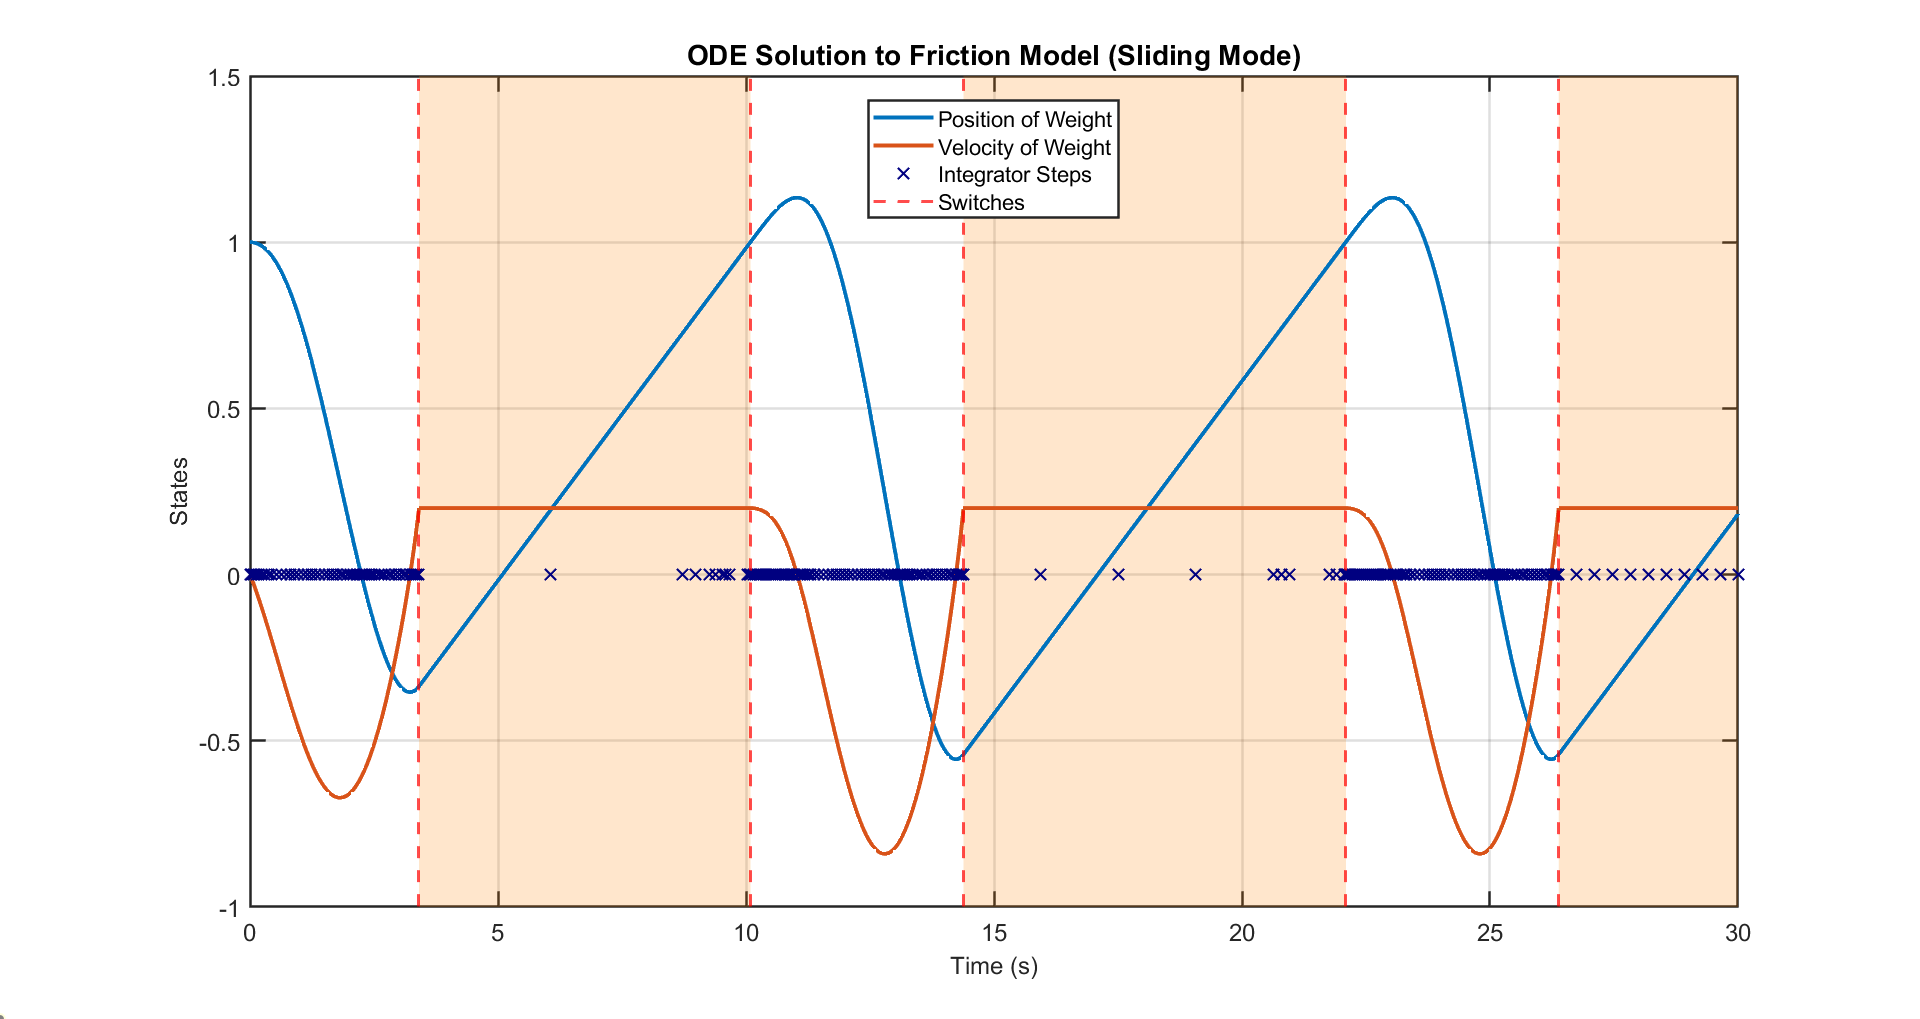
\includegraphics[width=1\linewidth]{Plots/task2a.png}
	\caption{Solution using Filippov mode of IFDIFF}
\end{figure}
\begin{figure}[H]
	\centering
	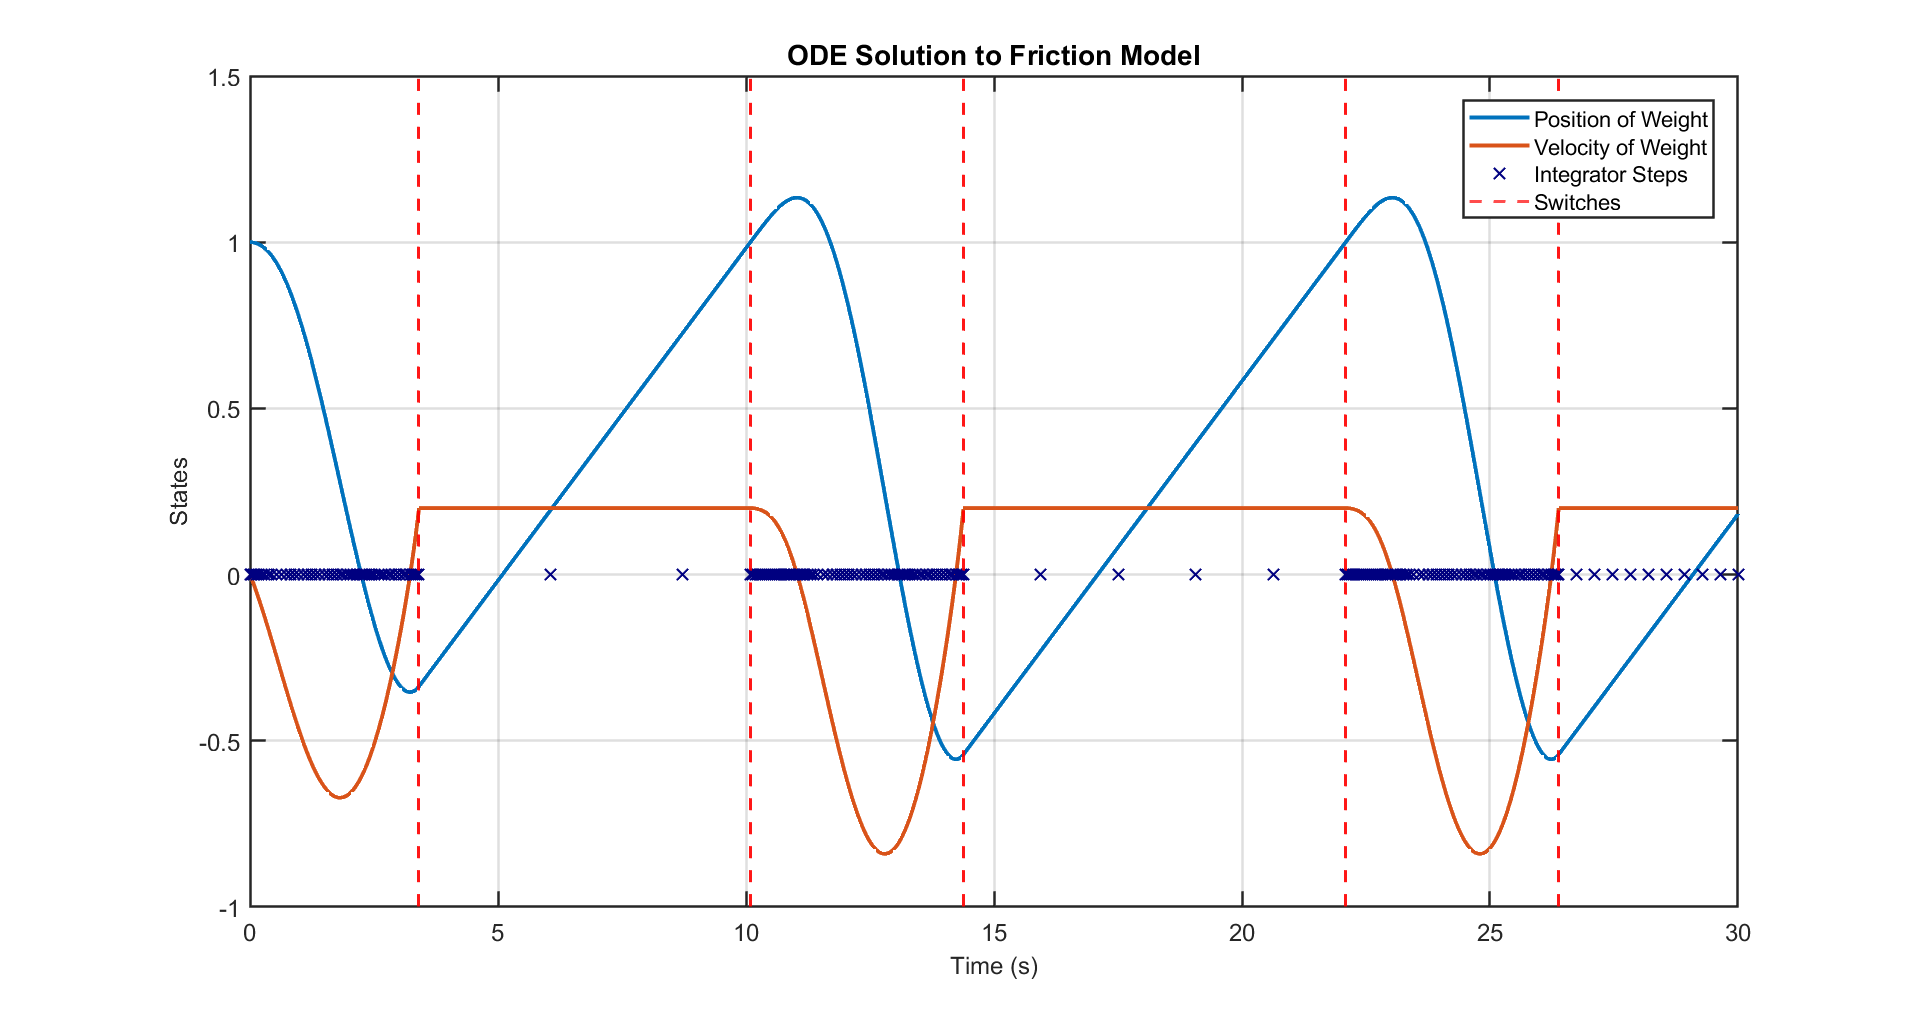
\includegraphics[width=1\linewidth]{Plots/task2c.png}
	\caption{Reference solution, using the more complicated RHS formulation}
\end{figure}
\begin{figure}[H]
	\centering
	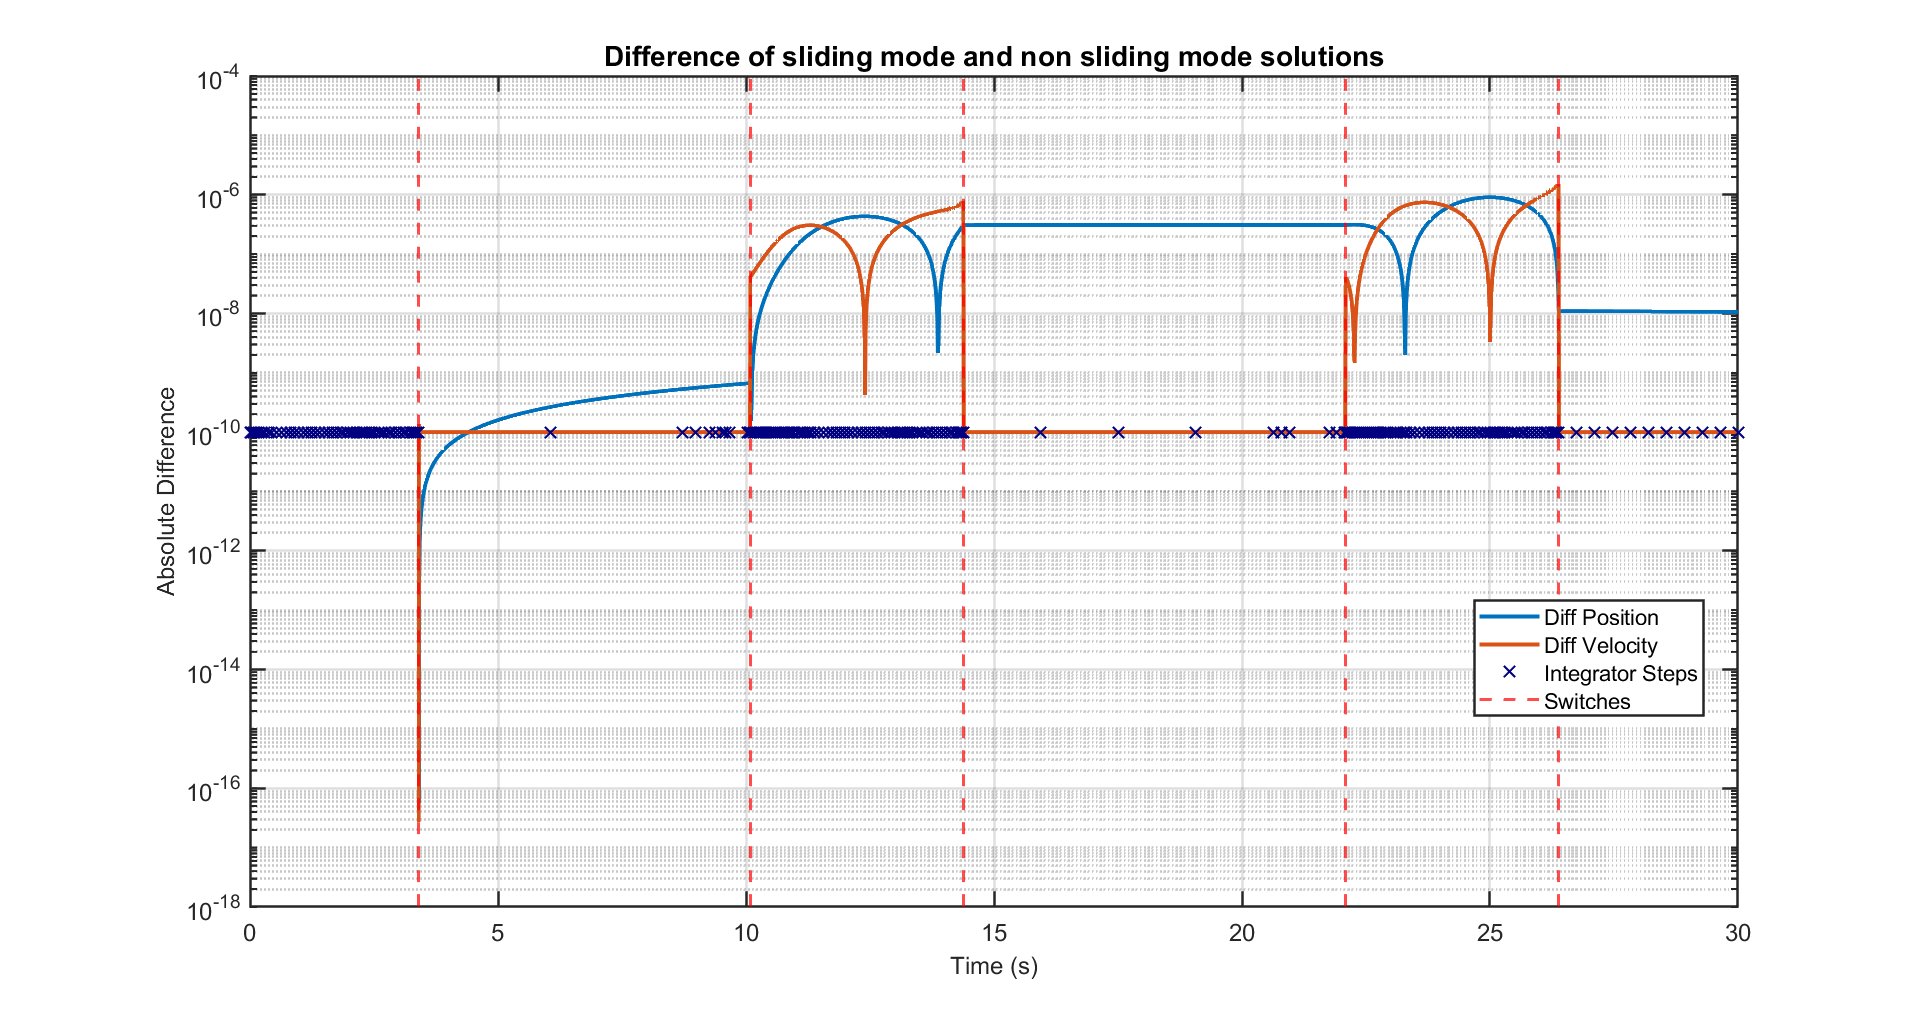
\includegraphics[width=1\linewidth]{Plots/task2_diff_plot.png}
	\caption{Difference Plot}
\end{figure}

 % Filippov Sliding Mode
\newpage
% % !TeX root = exercises_main.tex
\subsection*{Solution 3: Differential Algebraic Equations (DAE)}

Let's take a look at the following example for $t \in [0,3]$, $x = (x_1, x_2)^T$:
\begin{align*}
	(D) \quad
	\begin{cases}
		\dot{x}_ 1 = f(t,x,p) = 
		\begin{cases} 
			x_2, & \text{if } x_2 < p \\
			0, & \text{if } x_2 \geq p
		\end{cases} \\
		g(t,x,p) = x_1 + x_2 + x_1^3 + x_2^3 = 0 \\
		x_0 = (1.0, -1.0)^T, p = -0.5
	\end{cases}
\end{align*}

\begin{enumerate}[label=\alph*)]
	
	\item When we zoom in around the switching time $t_s \simeq 1.281$, we see that \lstinline|ode15s| does not notice the switch but instead fits a polynomial where the dynamics change.
\end{enumerate}

Plots for reference:
\begin{figure}[!h]
	\centering
	\includegraphics[width=\linewidth]{Plots/task3_plot.eps}
	\caption{Plot for c)}
\end{figure}
\begin{figure}[!h]
	\centering
	\includegraphics[width=\linewidth]{Plots/task3_close.eps}
	\caption{Zoomed in plot for c)}
\end{figure}
 % DAEs
\newpage
%% !TeX root = solutions_main.tex
\section*{Task 4: Solution}
\begin{enumerate}[label=\alph*)]
    \item\label{item:task4a} The maximum size of the population approaches $C = 1$ asymptotically. The population grows fastest when $P(t) = \frac{C}{2}$. \\\\
    \textbf{File:} \texttt{rhsTask4.m}
    \begin{lstlisting}
function dy = rhsTask4(~, y, p)
r = 2;
C = 1;

P = y(1);

dP = r.*P .* (1 - P./C);
dy = dP;
end
    \end{lstlisting}
    \textbf{File:} \texttt{runTask4.m}
    \begin{lstlisting}
%% Subtask a) and b)
%% Setup problem
tspan = [0, 5];
y0 = 0.1;

T = 0.5;
alpha = 0.5;
p = [T, alpha];

rhs = @rhsTask4;
integrator = @ode45;
optsIntegrator = odeset('AbsTol', 1e-10, 'RelTol', 1e-8);
datahandle = prepareDatahandleForIntegration(rhs, 'integrator', integrator, 'options', optsIntegrator);

%% Solve
solution = solveODE(datahandle, tspan, y0, p);

%% Plot solution
plotPopulation(solution);
    \end{lstlisting}
    \begin{figure}[H]
        \centering
        
\includegraphics[width=\textwidth]{Plots/task4a}
        \caption{Population plot for subtask \ref{item:task4a}}
    \end{figure}

    \item\label{item:task4b} If the parameters are set such that an actual harvest occurs, then the maximum population is equal to the harvest threshold $T$. Otherwise, the maximum size of the population approaches $C = 1$ asymptotically as before.\\\\
    \textbf{File:} \texttt{rhsTask4.m}
    \begin{lstlisting}
function dy = rhsTask4(~, y, p)
r = 2;
C = 1;

T     = p(1);
alpha = p(2);
P = y(1);

dP = r.*P .* (1 - P./C);
dH = 0;
dy = [dP; dH];

harvestCondition = P - T;
if ifdiff_jumpif(harvestCondition, 1)
    harvest = alpha .* P;
    jump = [-harvest; harvest];
    ifdiff_update(jump);
end
end
    \end{lstlisting}
    \textbf{File:} \texttt{runTask4.m}
    \begin{lstlisting}
%% Subtask a) and b)
%% Setup problem
tspan = [0, 5];
y0 = [0.1; 0];

T = 0.5;
alpha = 0.5;
p = [T, alpha];

rhs = @rhsTask4;
integrator = @ode45;
optsIntegrator = odeset('AbsTol', 1e-10, 'RelTol', 1e-8);
datahandle = prepareDatahandleForIntegration(rhs, 'integrator', integrator, 'options', optsIntegrator);

%% Solve
solution = solveODE(datahandle, tspan, y0, p);

%% Plot solution
plotPopulation(solution);
    \end{lstlisting}
    \begin{figure}[H]
        \centering
        
\includegraphics[width=\textwidth]{Plots/task4b}
        \caption{Population plot for subtask \ref{item:task4b}}
    \end{figure}

    \item\label{item:task4c} If $T = 0$, then a harvest will never trigger because the population starts at $P(0) = 0.1 > T = 0$ and thus never crosses the threshold $T = 0$. Similarly, if $T = C$, then a harvest also never triggers because the population merely approaches $T = C$ asymptotically, but may never reach and cross it.
    
    If $\alpha = 0$, then harvests may or may not trigger depending on the value of $T$, but will never have any effect on the solution because the proportion of the population extracted from the pond is always zero.
    
    If $\alpha = 1$ and a harvest occurs (i.e.~if $P(0) < T < C$), then the entire population will be depleted at the first harvest. The population remains at zero from that point onward.\\\\
    \textbf{File:} \texttt{runTask4.m}
    \begin{lstlisting}
%% Subtask c)
%% Solve for multiple parameters
solutionFunc = @(p) solveODE(datahandle, tspan, y0, p);

solutionGrid = solveOnGrid(solutionFunc);

%% Plot solution for multiple parameters
plotPopulationGrid(solutionGrid);
    \end{lstlisting}
    \begin{figure}[H]
        \centering
        
\includegraphics[width=\textwidth]{Plots/task4c}
        \caption{Population grid plot for subtask \ref{item:task4c}}
    \end{figure}

    \item\label{item:task4d} If $T = 0$, $T = C$ or $\alpha = 0$, then no actual harvests occur, so the objective function is determined only by the population at the end of the time interval, which will be approximately equal to $C = 1$.
    
    If $\alpha = 1$ and a harvest occurs (i.e.~if $P(0) < T < C$), then the entire population will be depleted at the first harvest, so the objective function is determined only by the amount harvested then, which will be equal to $T$, since $P(t) = T$ at the time of the harvest.

    The parameters which maximimze the objective function on the grid are $T = 0.5$ and $\alpha = 0.25$. \\ \\
    \textbf{File:} \texttt{runTask4.m}
    \begin{lstlisting}
%% Subtask d)
%% Compute objective
objectiveFunc = @(solution) sum(solution.y(:, end));

objectiveGrid = arrayfun(objectiveFunc, solutionGrid);

%% Plot objective
plotObjective(solutionGrid, objectiveGrid);
    \end{lstlisting}
    \begin{figure}[H]
        \centering
        
\includegraphics[width=\textwidth]{Plots/task4d}
        \caption{Objective function plot for subtask \ref{item:task4d}}
    \end{figure}

    \item\label{item:task4e} At the parameters which maximize the objective function on the grid, namely $T = 0.5$ and $\alpha = 0.25$, the gradient approximately points in the direction $d = (0.07, -0.02)$, which implies that we may achieve an even bigger value for the objective function by increasing the harvest threshold from $T = 0.5$ and reducing the harvest ratio from $\alpha = 0.25$. \\ \\
    \textbf{File:} \texttt{runTask4.m}
    \begin{lstlisting}
%% Subtask e)
%% Compute gradient
function g = computeGradient(datahandle, solution)
sensitivity = generateSensitivityFunction(datahandle, solution, 'calcGy', false);
Gp = sensitivity(solution.x(end)).Gp;
dP = Gp(1, :);
dH = Gp(2, :);
g = dP + dH;
end
gradientFunc = @(solution) computeGradient(datahandle, solution);

gradientGrid = arrayfun(gradientFunc, solutionGrid, 'UniformOutput', false);

%% Plot gradient
plotGradient(solutionGrid, objectiveGrid, gradientGrid)
    \end{lstlisting}
    \begin{figure}[H]
        \centering
        
\includegraphics[width=\textwidth]{Plots/task4e}
        \caption{Gradient plot for subtask \ref{item:task4e}}
    \end{figure}

    \item\label{item:task4f} After the first harvest, the population is strictly bound to the interval $J = [T, T - \alpha T]$. The midpoint of this interval is $m = T - \frac{(T - (T - \alpha T))}{2} = T(1 - \frac{\alpha}{2})$. For the optimal parameters $T^* \approx 0.56$ and $\alpha^* \approx 0.2$ the midpoint is located at approximately $m^* \approx 0.5 = \frac{C}{2}$.
    
    This behavior is not coincidental: Each fish produced over the time interval will be added to the value of the objective function, either as part of a harvest, or at the end of the time interval when the pond is emptied. In other words, fish that have been produced can never disappear. Therefore, to maximize the total amount of fish produced, it is sufficient to maximize the population growth over the entire time interval. The population growth is maximal when the population is at half of the total capacity of the pond, i.e. $P(t) = \frac{C}{2}$. The population growth decreases symmetrically as the population distances itself from the optimal point. Thus, our goal is to keep the population as close to the optimal point $\frac{C}{2}$ as possible.
    
    We know that our choice of parameters $T$ and $\alpha$ will constrain the population to the interval $J = [T, T - \alpha T]$. Since the population growth decreases quadratically with the distance of the population from the optimal point, we should choose $T$ and $\alpha$, s.t.~the interval $J$ has minimal length and is centered at $\frac{C}{2}$. Thus, choosing $\alpha^* = 0.2$ will minimize the length of the interval (under the constraint $\alpha \geq 0.2$). The optimal harvest threshold $T^*$ can then be obtained by enforcing $m^* = T^*(1 - \frac{\alpha^*}{2}) = \frac{C}{2}$ which yields $T^* = \frac{C}{2-\alpha^*} \approx 0.56$. This matches the numerical results obtained by the optimizer.\\ \\
    \textbf{File:} \texttt{runTask4.m}
    \begin{lstlisting}
%% Subtask f)
%% Optimize
function [f, g] = objWithGrad(p, solutionFunc, objectiveFunc, gradientFunc)
solution = solutionFunc(p);
f = -objectiveFunc(solution);
if nargout > 1
    g = -gradientFunc(solution);
end
end
optimizationFunc = @(p) objWithGrad(p, solutionFunc, objectiveFunc, gradientFunc);

[pOpt, objOpt] = optimizeParameters(optimizationFunc);
solutionOpt = solutionFunc(pOpt);

%% Plot optimal solution
fprintf('Optimal Parameters: T=%g, alpha=%g\n', pOpt);
fprintf('Optimal Total Harvest: %g\n', objOpt);

plotPopulation(solutionOpt);
    \end{lstlisting}
    \begin{figure}[H]
        \centering
        
\includegraphics[width=\textwidth]{Plots/task4f}
        \caption{Gradient plot for subtask \ref{item:task4f}}
    \end{figure}
\end{enumerate}
 % State Jumps

\end{document}
